\documentclass[11pt]{jarticle}
%
\usepackage[dvipdfmx]{graphicx}
\usepackage{amsmath}
\usepackage{amssymb}
\usepackage{bm}
\usepackage{float}
\usepackage{subfig}
\usepackage[justification=centering]{caption}
%
\addtolength{\textwidth}{40mm}
\addtolength{\oddsidemargin}{-20mm}
\addtolength{\evensidemargin}{-20mm}
\addtolength{\textheight}{15mm}
\addtolength{\topmargin}{-10mm}
%
\pagestyle{empty}
%
\title{研究進捗報告}
\author{里谷 佳紀}
%\date{\today}
\date{平成29年10月10日}
%
\begin{document}
%
\maketitle
\thispagestyle{empty}
%
\section{研究全体の目標}
与えられた頂点数と次数をもつ正則グラフのうち,Cerfらの平均頂点間距離の
下界\cite{Cerf1974}と一致する平均頂点間距離をもつグラフが存在するかを
判定する方法を開発する.また,既存の方法\cite{Yamamoto2016}と比較する
ことにより,新方法の有用性を検証する.

\section{前回打ち合わせ時に定めた短期目標}
\begin{enumerate}
\item 全域木予想の実験
\item 先行研究の調査
\end{enumerate}

\section{本日までの進捗状況}
\begin{enumerate}
\item 計算中である.計算できた頂点数と次数の組について,時間を計測した.
  結果を図\ref{fig:time}に示す.
\item Cerfらは,平均頂点間距離の下界\cite{Cerf1974}と一致する
  平均頂点間距離をもつグラフを,一般ムーアグラフ(Generalized Moore Graph)
  と定義した\cite{cerf1973computer}.
  後の成果から,ここで一般ムーアグラフに$2Q$以下の閉路が存在しないことと,
  直径が$Q+1$($R=0$の場合は$Q$)であることが示されたと推測できる.

  McKayとStantonは,次数が3で,頂点数が48と50の一般ムーアグラフが
  存在しないことを証明した\cite{mckay1979current}.
  Stantonらは,頂点数が44の一般ムーアグラフが存在しないことを証明した
  \cite{Stanton1980}.
  しかしながら,それらの方法は場合分けを細かくするもので,一般性は低い.

  Sampelsは,ケイリーグラフ(Cayley Graph)から平均頂点間距離が短いグラフを
  抜き出すことで,一般ムーアグラフを発見するアルゴリズムを開発した
  \cite{Sampels2004}.
\end{enumerate}

\begin{figure}[H]
  \centering

  \subfloat[$d=3$]{
    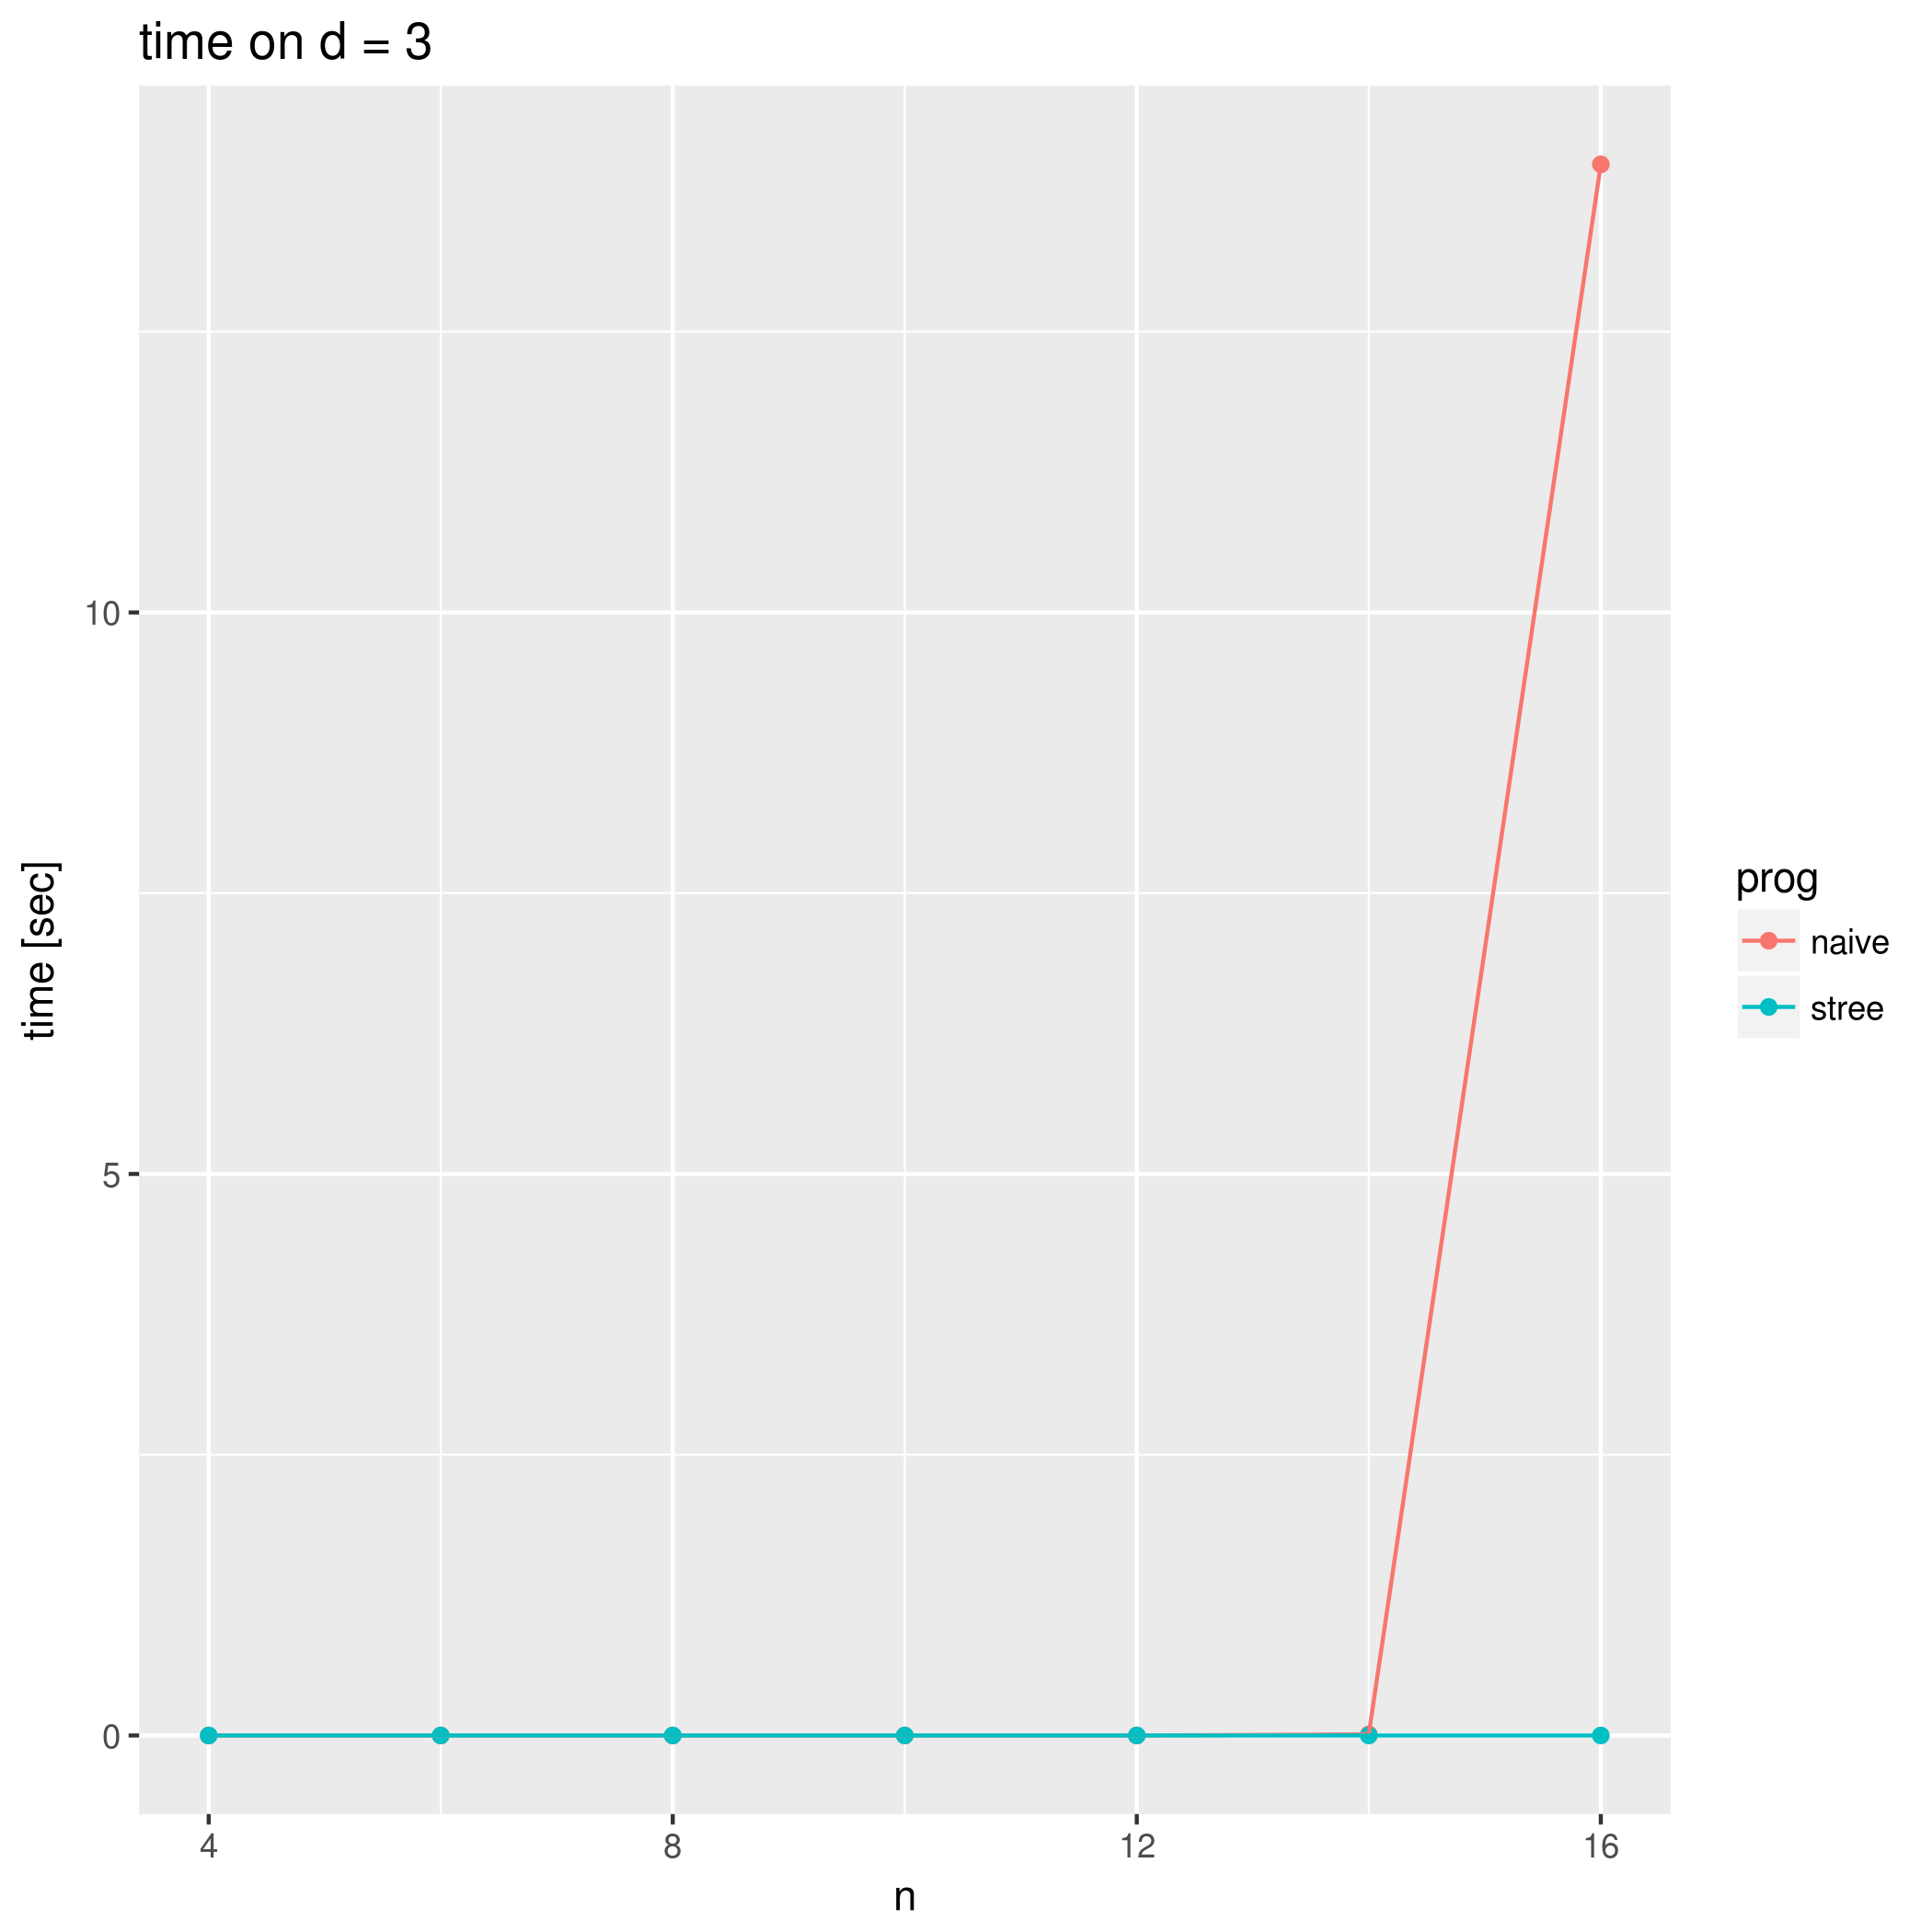
\includegraphics[width=.3\linewidth]{d3.png}
  }\hfill
  \subfloat[$d=4$]{
    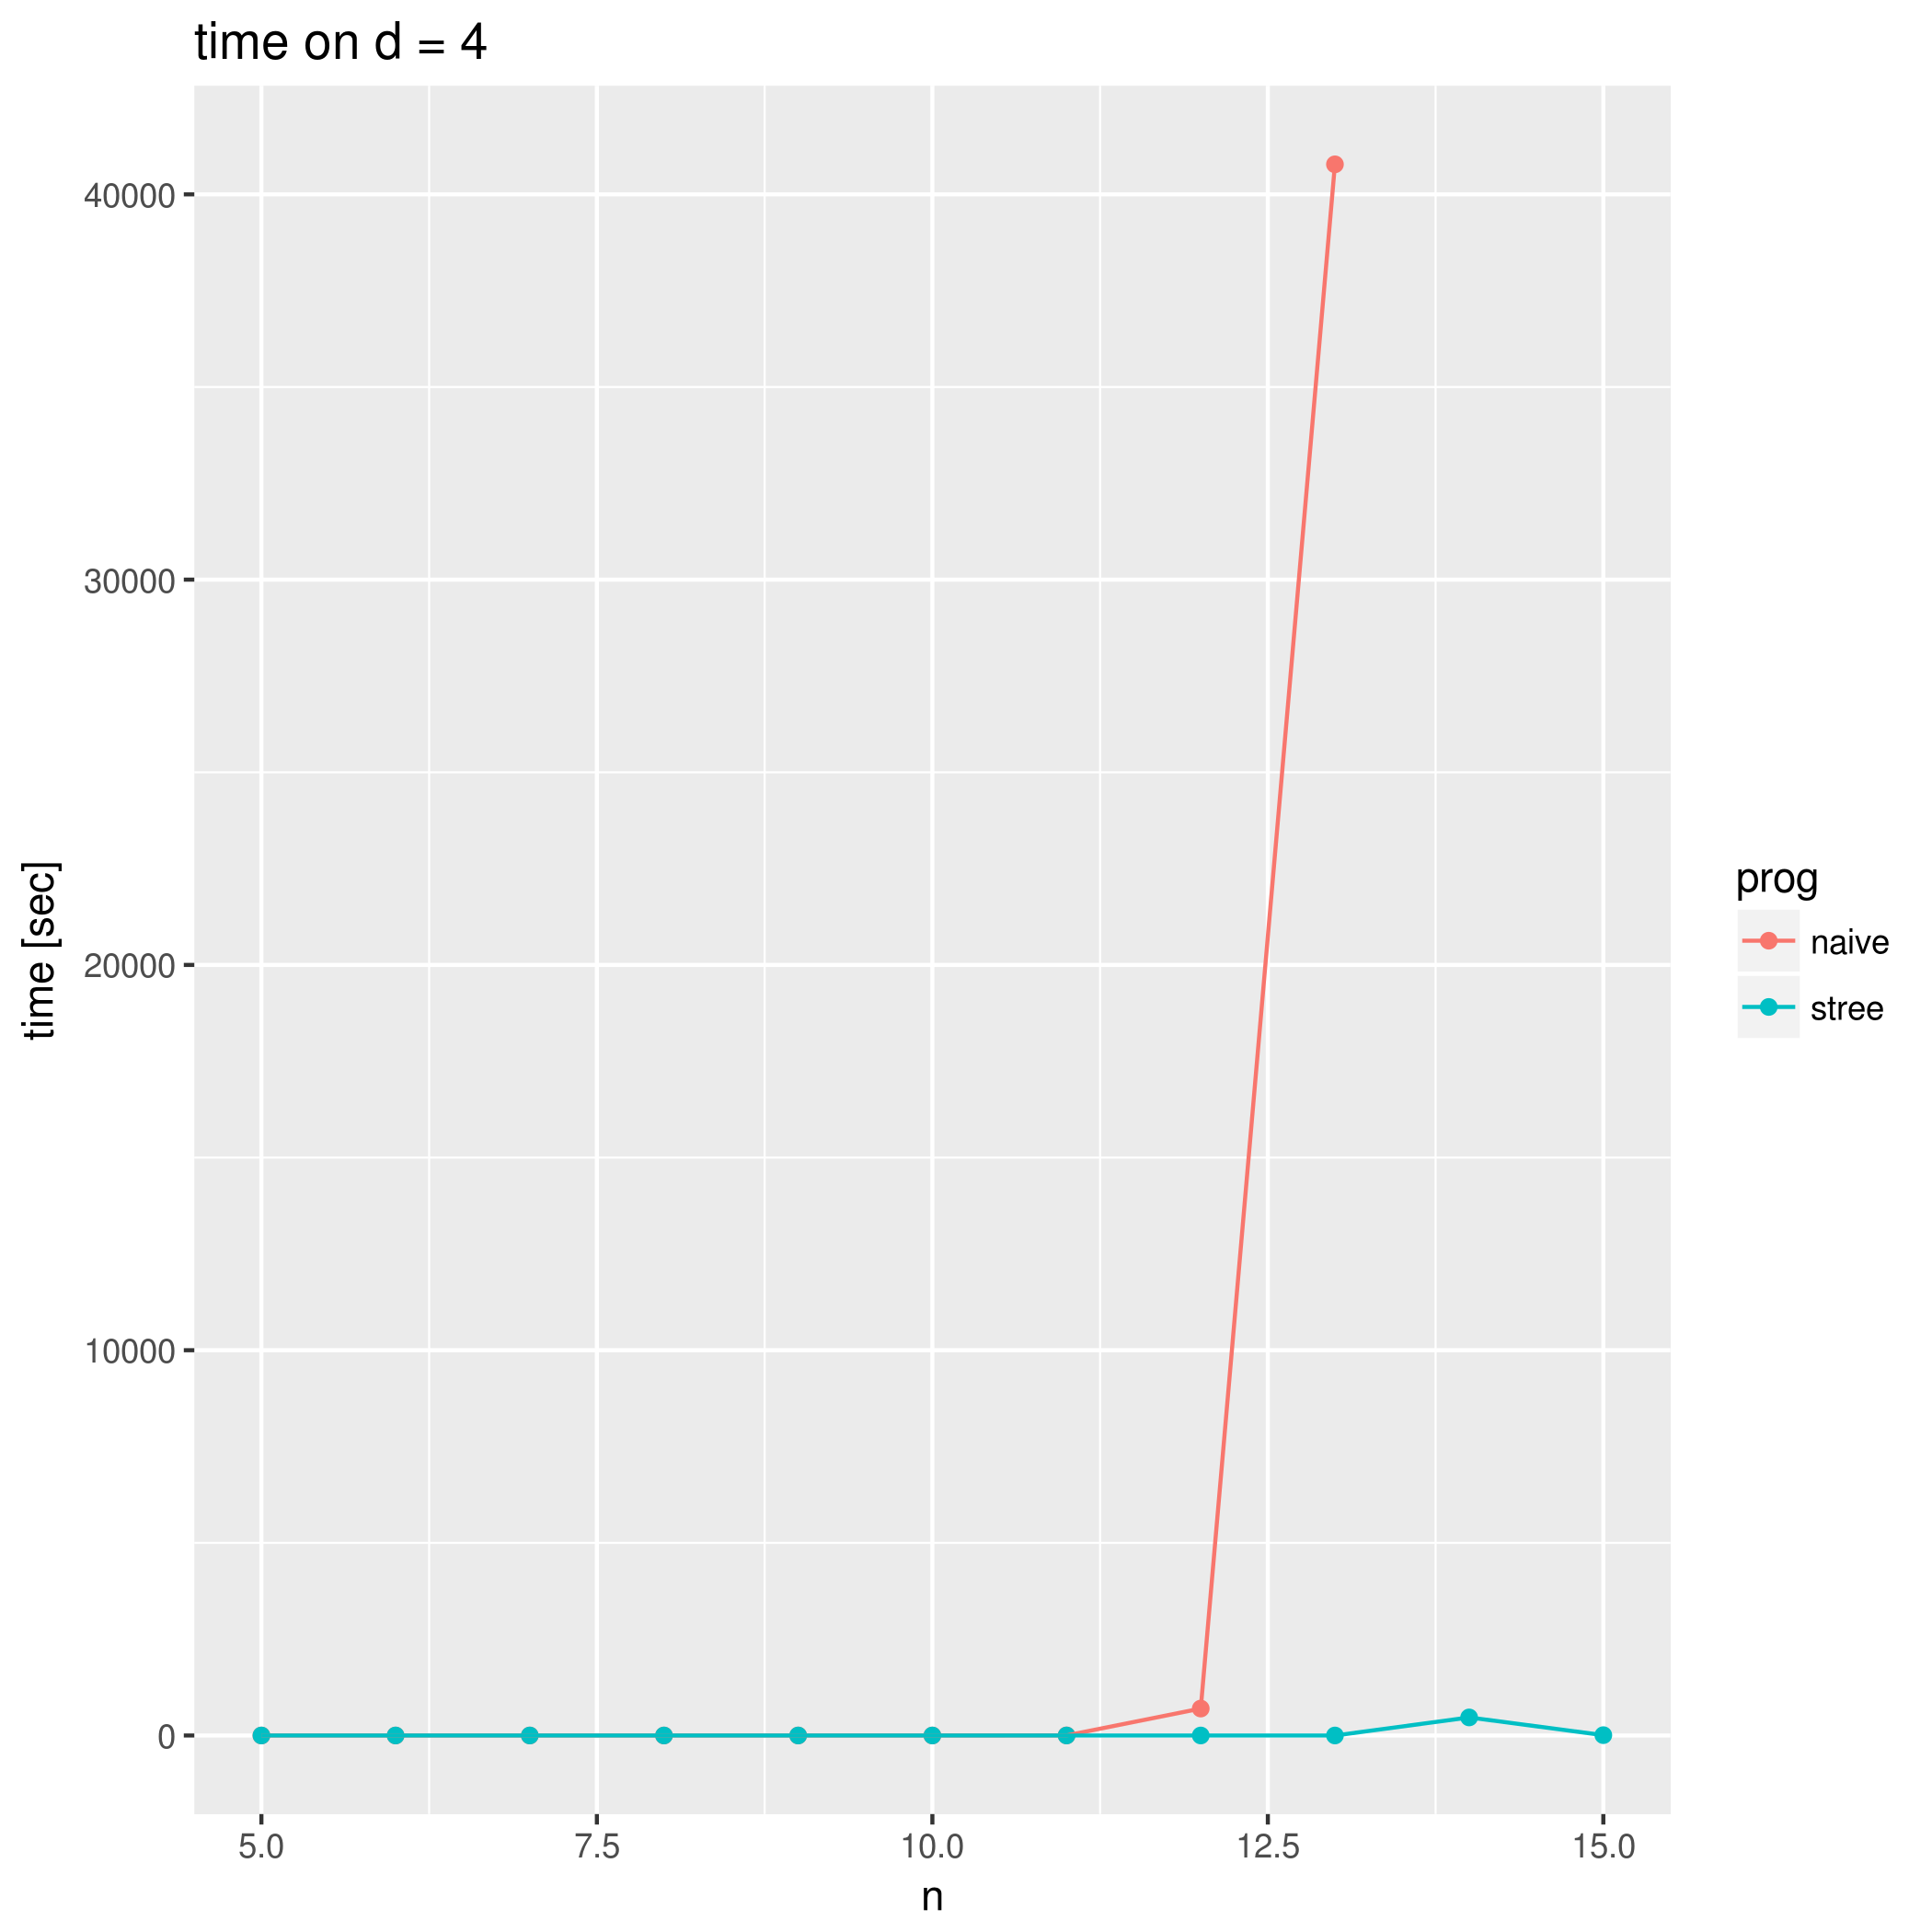
\includegraphics[width=.3\linewidth]{d4.png}
  }\hfill
  \subfloat[$d=5$]{
    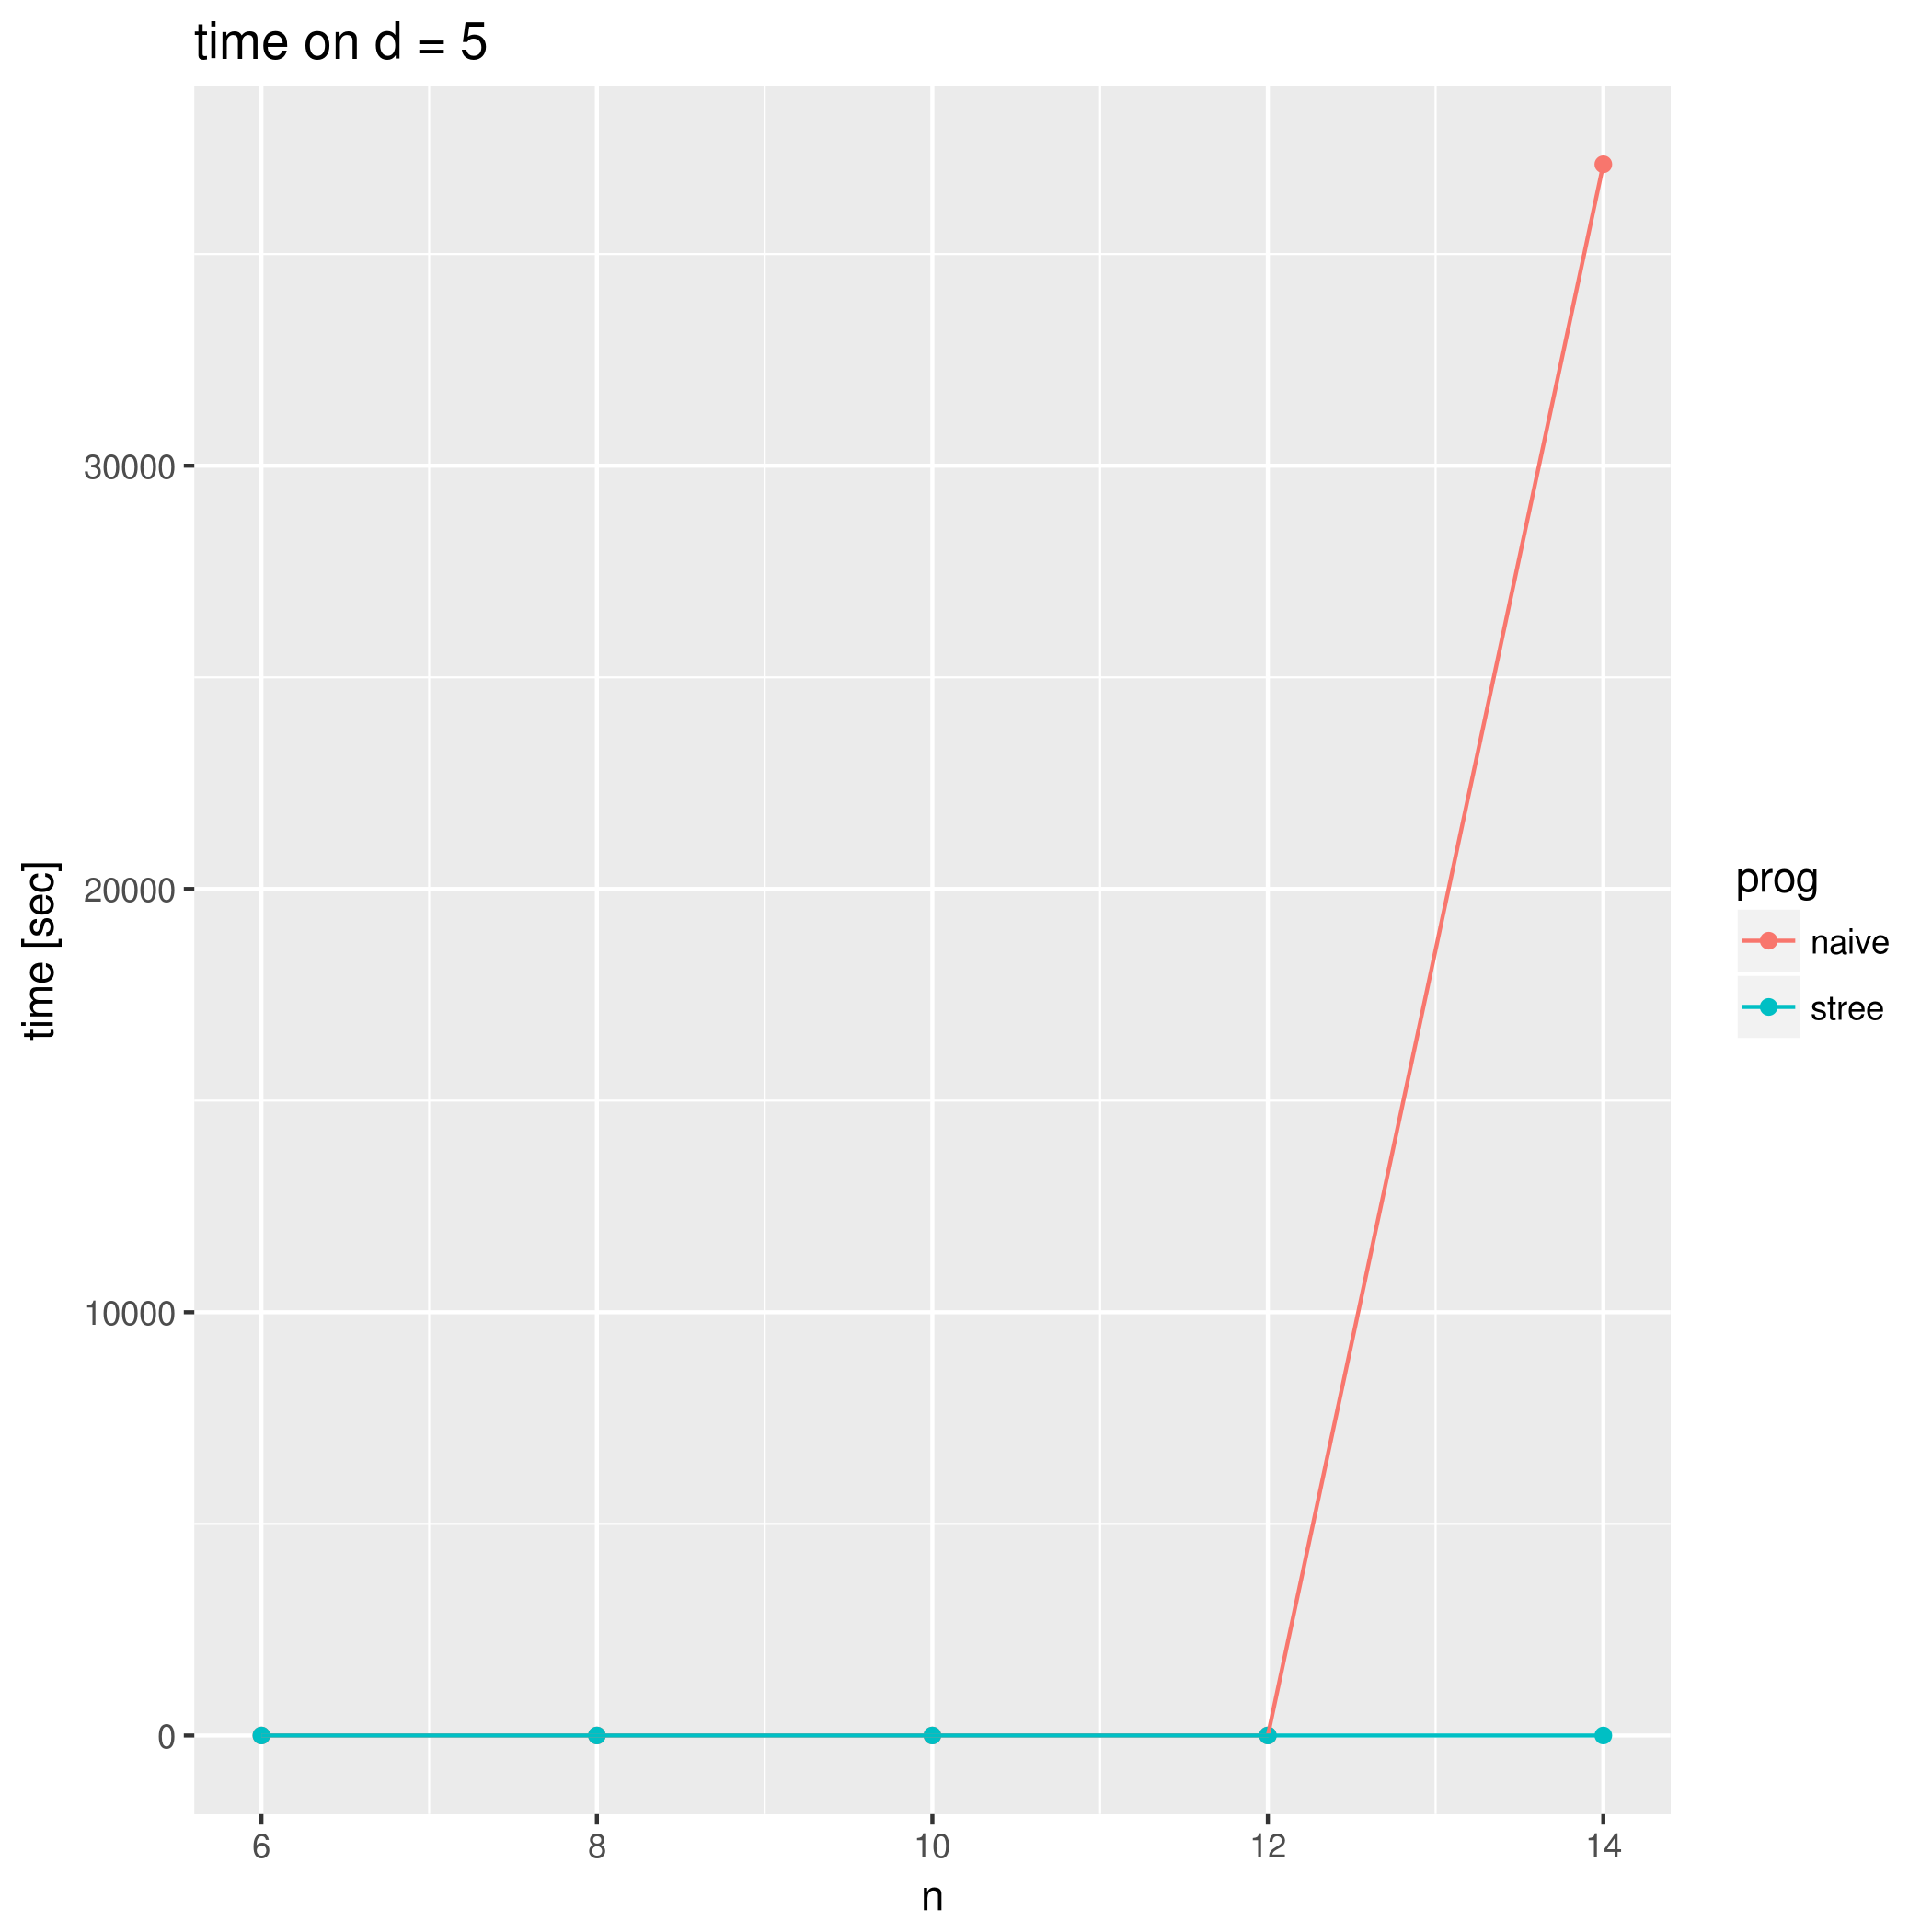
\includegraphics[width=.3\linewidth]{d5.png}
  }

  \caption{プログラムの実行時間の比較 \\
    横軸は頂点数を,縦軸は実行時間を表す.青い線は全域木から探索する方法を,
    赤い線は何も工夫しない方法を表す.
  }
  \label{fig:time}
\end{figure}

\bibliographystyle{junsrt}
\bibliography{refs}

\end{document}
